%! Author = zhiweizhang
%! Date = 10.06.25

\chapter{Results}\label{chapter:results}


\section{Binary Classification Results}

\subsection{Tabular Results}

The results for the binary classification task are summarized in ~\autoref{tab:binary-results}, which reports
accuracy, precision, recall, and F1-score for each evaluated model, \ac{AUC} and \ac{AP} for applicable models.

%! Author = zhiweizhang
%! Date = 10.06.25

\begin{table}[ht]
\centering
\resizebox{\textwidth}{!}{
\begin{tabular}{lccccc}
\toprule
\textbf{Model}                        & \textbf{Accuracy} & \textbf{Precision} & \textbf{Recall} & \textbf{F1-Score} & \textbf{AUC}   \\
\midrule
YOLOv11                               & 0.995             & 0.793              & 0.932           & 0.857             & 0.964          \\
ResNet                                & 0.996             & 0.843              & 0.893           & 0.867             & 0.945          \\
EfficientNet                          & 0.993             & 0.772              & 0.761           & 0.767             & 0.878          \\
ViT                                   & 0.997             & 0.910              & 0.893           & 0.901             & 0.945          \\
Moondream                             & 0.718             & 0.046              & 1.000           & 0.088             & 0.857          \\
OpenCLIP                              & 0.314             & 0.013              & 0.639           & 0.025             & 0.474          \\
OpenCLIP + Logistic Regression        & 0.996             & 0.923              & 0.882           & 0.902             & 0.940          \\
OpenCLIP + SGDClassifier              & 0.996             & 0.924              & 0.880           & 0.901             & 0.939          \\
OpenCLIP + KNeighborsClassifier       & 0.996             & 0.895              & \textbf{0.936}  & 0.915             & \textbf{0.966} \\
OpenCLIP + SVC                        & \textbf{0.997}    & 0.948              & 0.929           & \textbf{0.939}    & 0.964          \\
OpenCLIP + DecisionTreeClassifier     & 0.987             & 0.674              & 0.742           & 0.706             & 0.867          \\
OpenCLIP + BaggingClassifier          & 0.989             & 0.744              & 0.717           & 0.730             & 0.856          \\
OpenCLIP + AdaBoostClassifier         & 0.994             & 0.901              & 0.791           & 0.842             & 0.894          \\
OpenCLIP + GradientBoostingClassifier & 0.993             & 0.879              & 0.801           & 0.838             & 0.899          \\
OpenCLIP + RandomForestClassifier     & 0.981             & \textbf{0.983}     & 0.097           & 0.177             & 0.548          \\
OpenCLIP + VotingClassifier           & 0.996             & 0.945              & 0.873           & 0.908             & 0.936          \\
\bottomrule
\end{tabular}
}
  \caption{Binary classification performance across different models. The best scores for each metric are highlighted in bold.}
\label{tab:binary-results}
\end{table}


\subsection{Visual Comparison}

To facilitate a clear visual comparison of model performance on the binary classification task, bar plots were
generated for all selected models, including \ac{YOLO}, \ac{ResNet}, EfficientNet, \ac{ViT}, Moondream, OpenCLIP, and
OpenCLIP combined with \ac{SVC}.

~\autoref{fig:model-accuracy}, \autoref{fig:model-precision}, \autoref{fig:model-recall}, and
\autoref{fig:model-f1-score} depict the performance metrics, with the y-axis of each figure representing a metric of
the classification results. These visualizations highlight trade-offs among models and assist in identifying
the most effective architectures.

For binary classification, \ac{ViT}, \ac{YOLO}, and OpenCLIP-based models paired with classical
classifiers—particularly \ac{SVC} and KNeighborsClassifier—demonstrated superior performance. Specifically, \ac{ViT} and
OpenCLIP + \ac{SVC} achieved the highest F1-scores of 0.901 and 0.939, respectively. Conversely, Moondream and the
base OpenCLIP model exhibited comparatively lower effectiveness.

Notably, \textbf{Moondream} significantly underperformed across all metrics. This likely stems from its
architectural and training objectives: Moondream is a vision-language model optimized for tasks such as caption
generation and dialogue, rather than image classification. Its decoding component, aligned with safety mechanisms,
may intentionally suppress or censor content related to hate symbols—including omitting, paraphrasing, or
generalizing textual outputs when prompted about Nazi iconography. Such behavior undermines reliability in
downstream classification tasks where semantic precision is essential. Furthermore, its visual encoder may lack the
granularity necessary to distinguish between visually similar yet semantically distinct symbols—such as swastikas
versus unrelated geometric designs.

Similarly, the \textbf{OpenCLIP model alone} showed limited classification capability. As OpenCLIP is trained
primarily for contrastive image-text retrieval, its raw embeddings—when used without fine-tuning or a dedicated
classifier—may not form well-separated decision boundaries between symbol classes. However, when paired with
classical classifiers such as \textbf{SVC} or \textbf{KNN}, performance improved substantially. This suggests that
while OpenCLIP embeddings capture semantically meaningful image features, they require further downstream
supervision to align with fine-grained classification objectives.

Potential reasons behind the varying performance of different models, including these observations, are further
examined in the ~\autofullref{chapter:discussion-and-analysis}.

%! Author = zhiweizhang
%! Date = 11.06.25

% Preamble
\begin{figure}[ht]
    \centering
    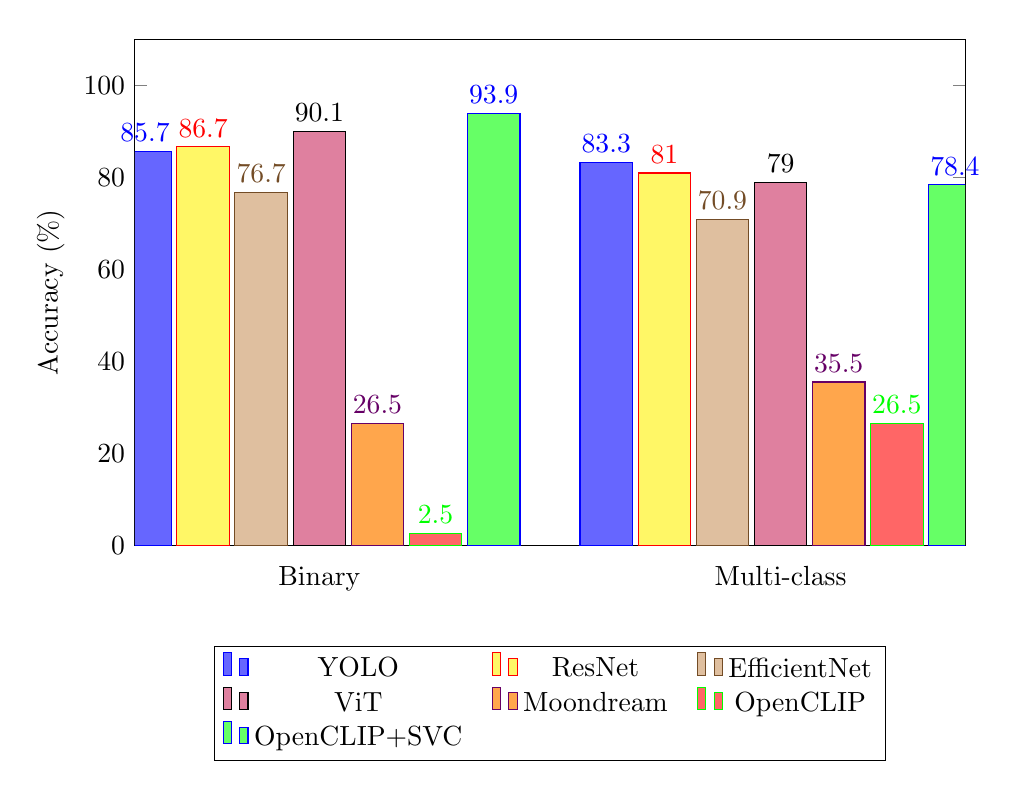
\begin{tikzpicture}
        \begin{axis}[
            ybar,
            bar width=19pt,
            width=\textwidth,
            height=8cm,
            enlarge x limits=0.4,
            ylabel={Accuracy (\%)},
            symbolic x coords={Binary, Multi-class},
            xtick=data,
            ymin=0.0, ymax=110.0,
            nodes near coords,
            nodes near coords align={vertical},
            major x tick style = transparent,
            legend style={
                at={(0.5,-0.2)},
                anchor=north,
                legend columns=3,
                /tikz/every even column/.append style={column sep=0.3cm}
            }
        ]
        \addplot+[style={fill=blue!60}]      coordinates {(Binary, 85.7) (Multi-class, 83.3)};
        \addplot+[style={fill=yellow!60}]    coordinates {(Binary, 86.7) (Multi-class, 81.0)};
        \addplot+[style={fill=brown!50}]     coordinates {(Binary, 76.7) (Multi-class, 70.9)};
        \addplot+[style={fill=purple!50}]    coordinates {(Binary, 90.1) (Multi-class, 79.0)};
        \addplot+[style={fill=orange!70}]    coordinates {(Binary, 26.5) (Multi-class, 35.5)};
        \addplot+[style={fill=red!60}]       coordinates {(Binary, 2.5) (Multi-class, 26.5)};
        \addplot+[style={fill=green!60}]     coordinates {(Binary, 93.9) (Multi-class, 78.4)};
        \legend{
            YOLO,
            ResNet,
            EfficientNet,
            ViT,
            Moondream,
            OpenCLIP,
            OpenCLIP+SVC
        }
        \end{axis}
    \end{tikzpicture}
    \caption{Comparison of F1-score values for all models on binary (left) and multi-class (right) classification tasks.}
    \label{fig:model-f1-score}
\end{figure}
%! Author = zhiweizhang
%! Date = 11.06.25

% Preamble
\begin{figure}[ht]
    \centering
    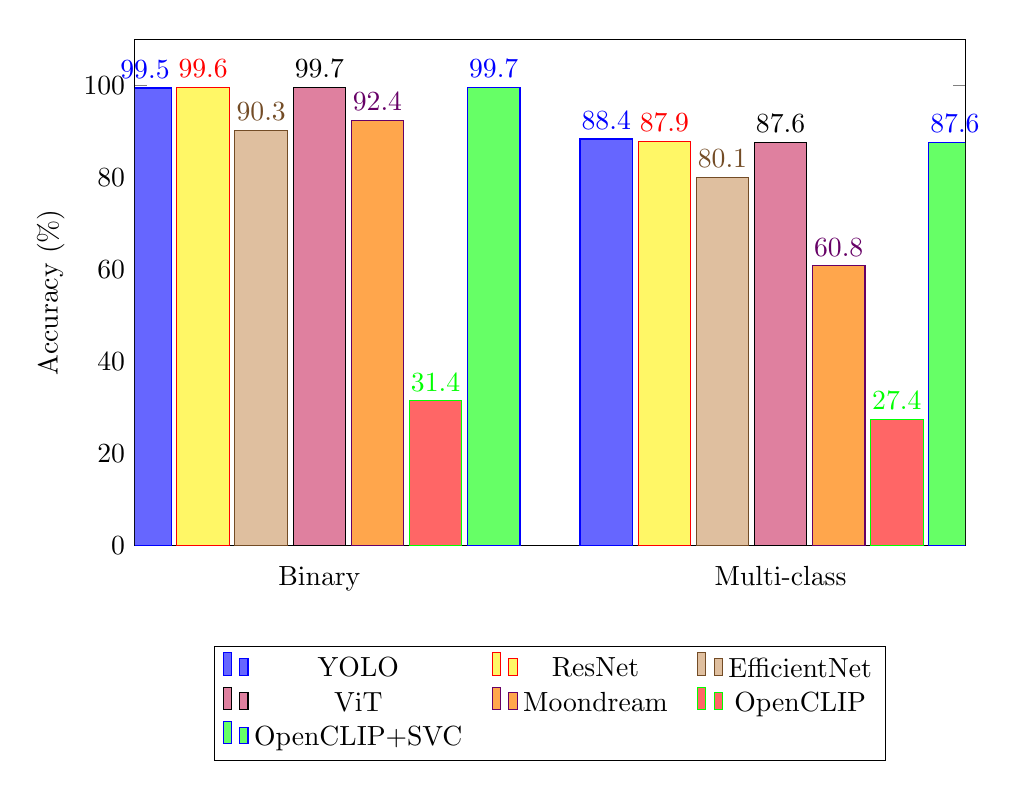
\begin{tikzpicture}
        \begin{axis}[
            ybar,
            bar width=19pt,
            width=\textwidth,
            height=8cm,
            enlarge x limits=0.4,
            ylabel={Accuracy (\%)},
            symbolic x coords={Binary, Multi-class},
            xtick=data,
            ymin=0.0, ymax=110.0,
            nodes near coords,
            nodes near coords align={vertical},
            major x tick style = transparent,
            legend style={
                at={(0.5,-0.2)},
                anchor=north,
                legend columns=3,
                /tikz/every even column/.append style={column sep=0.3cm}
            }
        ]
        \addplot+[style={fill=blue!60}]      coordinates {(Binary, 99.5) (Multi-class, 88.4)};
        \addplot+[style={fill=yellow!60}]    coordinates {(Binary, 99.6) (Multi-class, 87.9)};
        \addplot+[style={fill=brown!50}]     coordinates {(Binary, 90.3) (Multi-class, 80.1)};
        \addplot+[style={fill=purple!50}]    coordinates {(Binary, 99.7) (Multi-class, 87.6)};
        \addplot+[style={fill=orange!70}]    coordinates {(Binary, 92.4) (Multi-class, 60.8)};
        \addplot+[style={fill=red!60}]       coordinates {(Binary, 31.4) (Multi-class, 27.4)};
        \addplot+[style={fill=green!60}]     coordinates {(Binary, 99.7) (Multi-class, 87.6)};
        \legend{
            YOLO,
            ResNet,
            EfficientNet,
            ViT,
            Moondream,
            OpenCLIP,
            OpenCLIP+SVC
        }
        \end{axis}
    \end{tikzpicture}
    \caption{Comparison of accuracy scores for all models on binary (left) and multi-class (right) classification tasks.}
    \label{fig:model-accuracy}
\end{figure}
%! Author = zhiweizhang
%! Date = 11.06.25

% Preamble
\begin{figure}[ht]
    \centering
    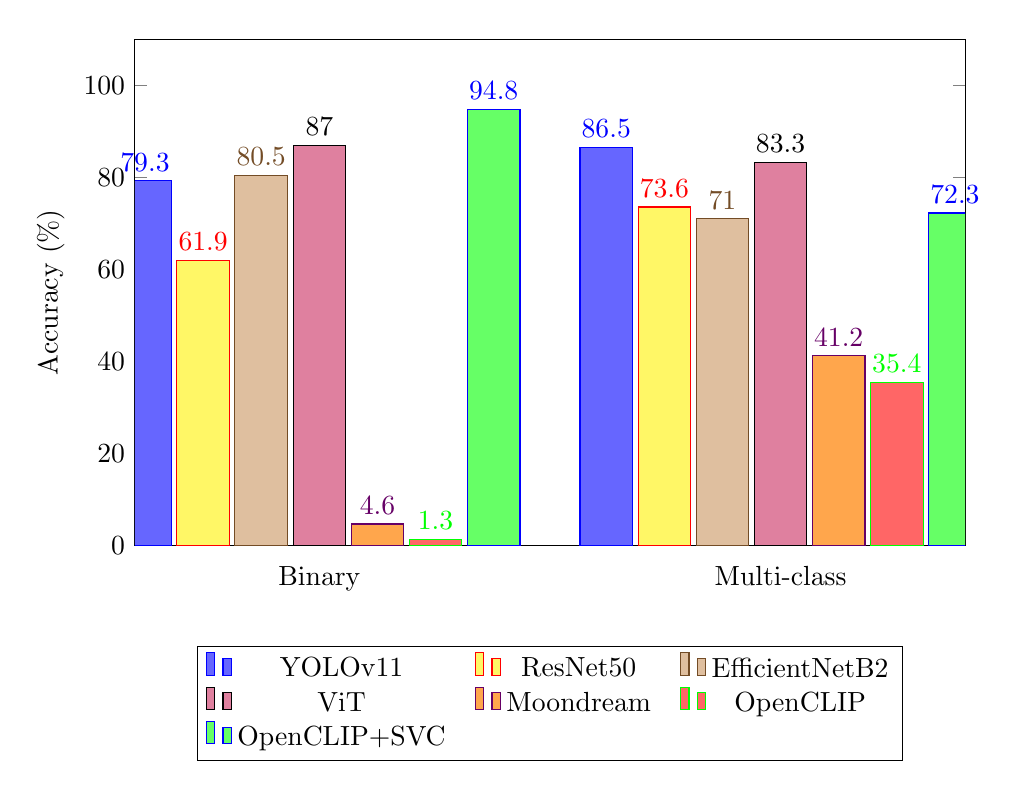
\begin{tikzpicture}
        \begin{axis}[
            ybar,
            bar width=19pt,
            width=\textwidth,
            height=8cm,
            enlarge x limits=0.4,
            ylabel={Accuracy (\%)},
            symbolic x coords={Binary, Multi-class},
            xtick=data,
            ymin=0.0, ymax=110.0,
            nodes near coords,
            nodes near coords align={vertical},
            major x tick style = transparent,
            legend style={
                at={(0.5,-0.2)},
                anchor=north,
                legend columns=3,
                /tikz/every even column/.append style={column sep=0.3cm}
            }
        ]
        \addplot+[style={fill=blue!60}]      coordinates {(Binary, 79.3) (Multi-class, 86.5)};
        \addplot+[style={fill=yellow!60}]    coordinates {(Binary, 61.9) (Multi-class, 73.6)};
        \addplot+[style={fill=brown!50}]     coordinates {(Binary, 80.5) (Multi-class, 71.0)};
        \addplot+[style={fill=purple!50}]    coordinates {(Binary, 87.0) (Multi-class, 83.3)};
        \addplot+[style={fill=orange!70}]    coordinates {(Binary, 4.6) (Multi-class, 41.2)};
        \addplot+[style={fill=red!60}]       coordinates {(Binary, 1.3) (Multi-class, 35.4)};
        \addplot+[style={fill=green!60}]     coordinates {(Binary, 94.8) (Multi-class, 72.3)};
        \legend{
            YOLOv11,
            ResNet50,
            EfficientNetB2,
            ViT,
            Moondream,
            OpenCLIP,
            OpenCLIP+SVC
        }
        \end{axis}
    \end{tikzpicture}
    \caption{Classification precision of selected models for binary and multi-class tasks.}
    \label{fig:model-precision}
\end{figure}
%! Author = zhiweizhang
%! Date = 11.06.25

% Preamble
\begin{figure}[ht]
    \centering
    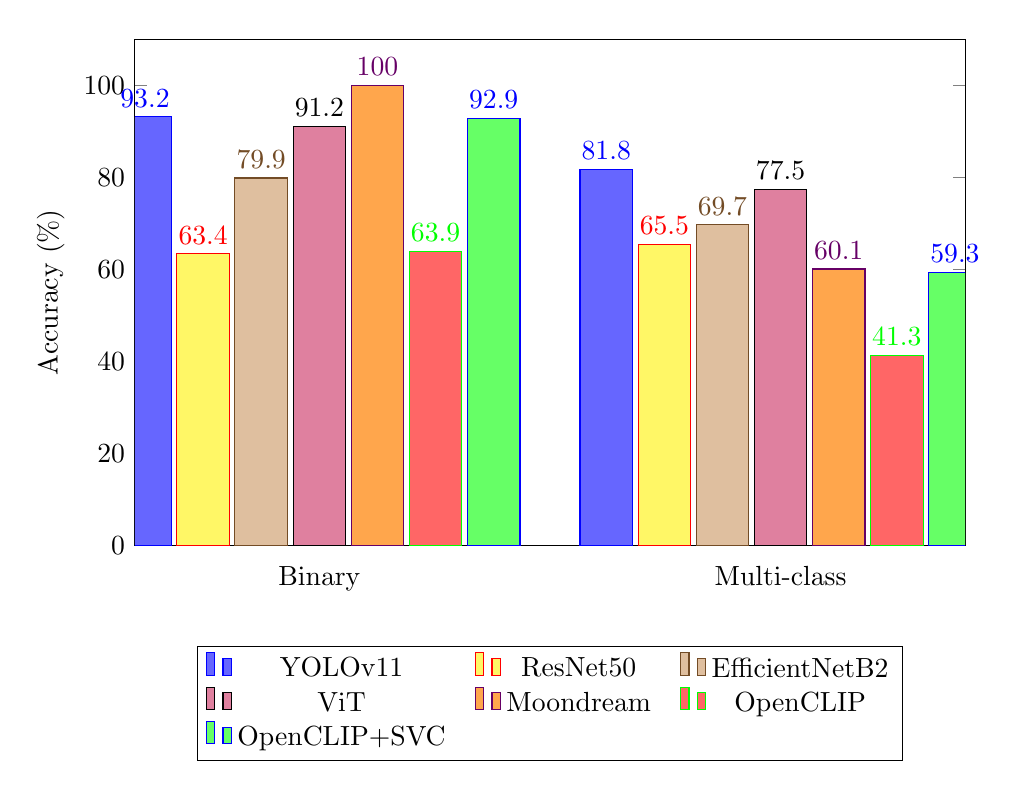
\begin{tikzpicture}
        \begin{axis}[
            ybar,
            bar width=19pt,
            width=\textwidth,
            height=8cm,
            enlarge x limits=0.4,
            ylabel={Accuracy (\%)},
            symbolic x coords={Binary, Multi-class},
            xtick=data,
            ymin=0.0, ymax=110.0,
            nodes near coords,
            nodes near coords align={vertical},
            major x tick style = transparent,
            legend style={
                at={(0.5,-0.2)},
                anchor=north,
                legend columns=3,
                /tikz/every even column/.append style={column sep=0.3cm}
            }
        ]
        \addplot+[style={fill=blue!60}]      coordinates {(Binary, 93.2) (Multi-class, 81.8)};
        \addplot+[style={fill=yellow!60}]    coordinates {(Binary, 63.4) (Multi-class, 65.5)};
        \addplot+[style={fill=brown!50}]     coordinates {(Binary, 79.9) (Multi-class, 69.7)};
        \addplot+[style={fill=purple!50}]    coordinates {(Binary, 91.2) (Multi-class, 77.5)};
        \addplot+[style={fill=orange!70}]    coordinates {(Binary, 100.0) (Multi-class, 60.1)};
        \addplot+[style={fill=red!60}]       coordinates {(Binary, 63.9) (Multi-class, 41.3)};
        \addplot+[style={fill=green!60}]     coordinates {(Binary, 92.9) (Multi-class, 59.3)};
        \legend{
            YOLOv11,
            ResNet50,
            EfficientNetB2,
            ViT,
            Moondream,
            OpenCLIP,
            OpenCLIP+SVC
        }
        \end{axis}
    \end{tikzpicture}
    \caption{Comparison of recall scores for all models on binary (left) and multi-class (right) classification tasks.}
    \label{fig:model-recall}
\end{figure}
\newpage

\subsection{Confusion Matrices}

Confusion matrices for the binary classification task are shown in~\autoref{fig:confusion-matrix-binary}. Each
matrix represents a model trained to distinguish images as either \textbf{Nazi} or \textbf{Non-Nazi}.

The evaluated models include \ac{YOLO}, EfficientNet, \ac{ResNet}, \ac{ViT}, and an OpenCLIP encoder paired with a
support vector classifier (SVC). These matrices visualize each model's prediction distribution by presenting true
positives, true negatives, false positives, and false negatives.

In general, most models achieved strong diagonal dominance, indicating successful classification of both Nazi and
non-Nazi symbols. Notably:

\begin{itemize}
\item \textbf{YOLO} and \textbf{EfficientNet} achieved relatively balanced true positive and true negative counts,
reflecting consistent performance across both classes.
\item \textbf{ResNet} and \textbf{ViT} also performed reliably, with lower false positive rates, suggesting a
cautious approach that reduces mislabeling benign symbols as Nazi-related.
\item The \textbf{OpenCLIP+SVC} configuration showed improved class separation compared to raw OpenCLIP outputs,
confirming the importance of combining feature extractors with downstream classifiers.
\end{itemize}

However, misclassifications still occurred—particularly false negatives, where Nazi symbols were not detected. These
errors highlight the difficulty of classifying visually degraded, ambiguous, or stylistically subtle symbols, which
will be analyzed in depth in ~\autofullref{chapter:discussion-and-analysis}.

%! Author = zhiweizhang
%! Date = 13.06.25

% Preamble
\begin{figure}[ht]
    \begin{subfigure}[b]{0.45\textwidth}
    \centering
        \begin{tikzpicture}
            \begin{axis}[
                width=0.9\textwidth,
                colormap={bluewhite}{color=(white) rgb255=(90,96,191)},
                xlabel=Predicted,
                ylabel=Actual,
                xticklabels={Non-Nazi, Nazi}, % changed
                xtick={0,...,1}, % changed
                xtick style={draw=none},
                yticklabels={Non-Nazi, Nazi}, % changed
                ytick={0,...,1}, % changed
                ytick style={draw=none},
                enlargelimits=false,
                colorbar,
                point meta min=0,
                point meta max=200,
                xticklabel style={
                  text width=1cm,align=center
                },
                yticklabel style={
                  text width=1cm,align=center
                },
                nodes near coords={\pgfmathprintnumber\pgfplotspointmeta},
                nodes near coords style={
                    yshift=-7pt
                },
            ]
                \addplot[
                    matrix plot,
                    mesh/cols=2, % changed
                    point meta=explicit,
                    draw=gray
                ] table [meta=C, x=x, y=y, col sep=comma] {data/yolo-binary-confusion-matrix-data.csv};
            \end{axis}
        \end{tikzpicture}
        \caption{Confusion matrix of YOLO.}\label{fig:yolo-confusion-matrix-binary}
    \end{subfigure}
    \hfill
    \begin{subfigure}[b]{0.45\textwidth}
    \centering
        \begin{tikzpicture}
            \begin{axis}[
                width=0.9\textwidth,
                colormap={bluewhite}{color=(white) rgb255=(90,96,191)},
                xlabel=Predicted,
                ylabel=Actual,
                xticklabels={Non-Nazi, Nazi}, % changed
                xtick={0,...,1}, % changed
                xtick style={draw=none},
                yticklabels={Non-Nazi, Nazi}, % changed
                ytick={0,...,1}, % changed
                ytick style={draw=none},
                enlargelimits=false,
                colorbar,
                point meta min=0,
                point meta max=200,
                xticklabel style={
                  text width=1cm,align=center
                },
                yticklabel style={
                  text width=1cm,align=center
                },
                nodes near coords={\pgfmathprintnumber\pgfplotspointmeta},
                nodes near coords style={
                    yshift=-7pt
                },
            ]
                \addplot[
                    matrix plot,
                    mesh/cols=2, % changed
                    point meta=explicit,
                    draw=gray
                ] table [meta=C, x=x, y=y, col sep=comma] {data/efficientnet-binary-confusion-matrix-data.csv};
            \end{axis}
        \end{tikzpicture}
        \caption{Confusion matrix of EfficientNet.}\label{fig:efficient-confusion-matrix-binary}
    \end{subfigure}
    \hfill
    \begin{subfigure}[b]{0.45\textwidth}
    \centering
        \begin{tikzpicture}
            \begin{axis}[
                width=0.9\textwidth,
                colormap={bluewhite}{color=(white) rgb255=(90,96,191)},
                xlabel=Predicted,
                ylabel=Actual,
                xticklabels={Non-Nazi, Nazi}, % changed
                xtick={0,...,1}, % changed
                xtick style={draw=none},
                yticklabels={Non-Nazi, Nazi}, % changed
                ytick={0,...,1}, % changed
                ytick style={draw=none},
                enlargelimits=false,
                colorbar,
                point meta min=0,
                point meta max=200,
                xticklabel style={
                  text width=1cm,align=center
                },
                yticklabel style={
                  text width=1cm,align=center
                },
                nodes near coords={\pgfmathprintnumber\pgfplotspointmeta},
                nodes near coords style={
                    yshift=-7pt
                },
            ]
                \addplot[
                    matrix plot,
                    mesh/cols=2, % changed
                    point meta=explicit,
                    draw=gray
                ] table [meta=C, x=x, y=y, col sep=comma] {data/openclip_encoder-binary-confusion-matrix-data.csv};
            \end{axis}
        \end{tikzpicture}
        \caption{Confusion matrix of OpenCLIP encoder and SVC.}\label{fig:openclip-encoder-confusion-matrix-binary}
    \end{subfigure}
    \hfill
    \begin{subfigure}[b]{0.45\textwidth}
    \centering
        \begin{tikzpicture}
            \begin{axis}[
                width=0.9\textwidth,
                colormap={bluewhite}{color=(white) rgb255=(90,96,191)},
                xlabel=Predicted,
                ylabel=Actual,
                xticklabels={Non-Nazi, Nazi}, % changed
                xtick={0,...,1}, % changed
                xtick style={draw=none},
                yticklabels={Non-Nazi, Nazi}, % changed
                ytick={0,...,1}, % changed
                ytick style={draw=none},
                enlargelimits=false,
                colorbar,
                point meta min=0,
                point meta max=200,
                xticklabel style={
                  text width=1cm,align=center
                },
                yticklabel style={
                  text width=1cm,align=center
                },
                nodes near coords={\pgfmathprintnumber\pgfplotspointmeta},
                nodes near coords style={
                    yshift=-7pt
                },
            ]
                \addplot[
                    matrix plot,
                    mesh/cols=2, % changed
                    point meta=explicit,
                    draw=gray
                ] table [meta=C, x=x, y=y, col sep=comma] {data/resnet-binary-confusion-matrix-data.csv};
            \end{axis}
        \end{tikzpicture}
        \caption{Confusion matrix of ResNet.}\label{fig:resnet-encoder-confusion-matrix-binary}
    \end{subfigure}
    \hfill
    \begin{subfigure}[b]{0.45\textwidth}
    \centering
        \begin{tikzpicture}
            \begin{axis}[
                width=0.9\textwidth,
                colormap={bluewhite}{color=(white) rgb255=(90,96,191)},
                xlabel=Predicted,
                ylabel=Actual,
                xticklabels={Non-Nazi, Nazi}, % changed
                xtick={0,...,1}, % changed
                xtick style={draw=none},
                yticklabels={Non-Nazi, Nazi}, % changed
                ytick={0,...,1}, % changed
                ytick style={draw=none},
                enlargelimits=false,
                colorbar,
                point meta min=0,
                point meta max=200,
                xticklabel style={
                  text width=1cm,align=center
                },
                yticklabel style={
                  text width=1cm,align=center
                },
                nodes near coords={\pgfmathprintnumber\pgfplotspointmeta},
                nodes near coords style={
                    yshift=-7pt
                },
            ]
                \addplot[
                    matrix plot,
                    mesh/cols=2, % changed
                    point meta=explicit,
                    draw=gray
                ] table [meta=C, x=x, y=y, col sep=comma] {data/vit-binary-confusion-matrix-data.csv};
            \end{axis}
        \end{tikzpicture}
        \caption{Confusion matrix of ViT.}\label{fig:vit-encoder-confusion-matrix-binary}
    \end{subfigure}

    \caption{Confusion matrices illustrating classification results of the binary task for each evaluated model. The matrices display true positive, true negative, false positive, and false negative counts for the classes “Nazi” and “Non-Nazi.”}
    \label{fig:confusion-matrix-binary}
\end{figure}

\subsection{Receiver Operating Characteristic (ROC) and Precision-Recall (PR) Curves}

To further characterize model performance under class imbalance, \ac{ROC} and \ac{PR} curves were plotted for the
binary classification task.

~\autoref{fig:roc-curve} illustrates the \ac{ROC} curves, demonstrating the trade-off between true positive rate and
false positive rate across different thresholds. The \ac{AUC} values reported in ~\autoref{tab:binary-results}
correspond with the visual trends observed. Most models exhibit near-perfect AUC scores ($\geq$0.998), indicating strong
overall separability between Nazi and Non-Nazi classes.

~\autoref{fig:pr-curve} presents the \ac{PR} curves, which are particularly informative when evaluating classifiers
under imbalanced conditions. The area under the \ac{PR} curve (\ac{AP}) complements the \ac{AUC-ROC},
emphasizing each model's ability to retrieve relevant positive samples effectively. Models such as OpenCLIP +
Logistic Regression (\ac{AP} = 0.964), \ac{ViT} (\ac{AP} = 0.962), and OpenCLIP + SVC (unreported \ac{AP} but high F1)
demonstrate particularly strong precision-recall trade-offs. In contrast, models like EfficientNet and
DecisionTreeClassifier show notably lower AP scores (0.780 and 0.625 respectively), reflecting limitations in
correctly retrieving positive instances under imbalance.

These curves and scores provide a nuanced view of classification confidence and retrieval quality beyond accuracy,
particularly important in safety-critical applications where false positives or false negatives may carry different risks.

\begin{figure}[ht]
  \centering
  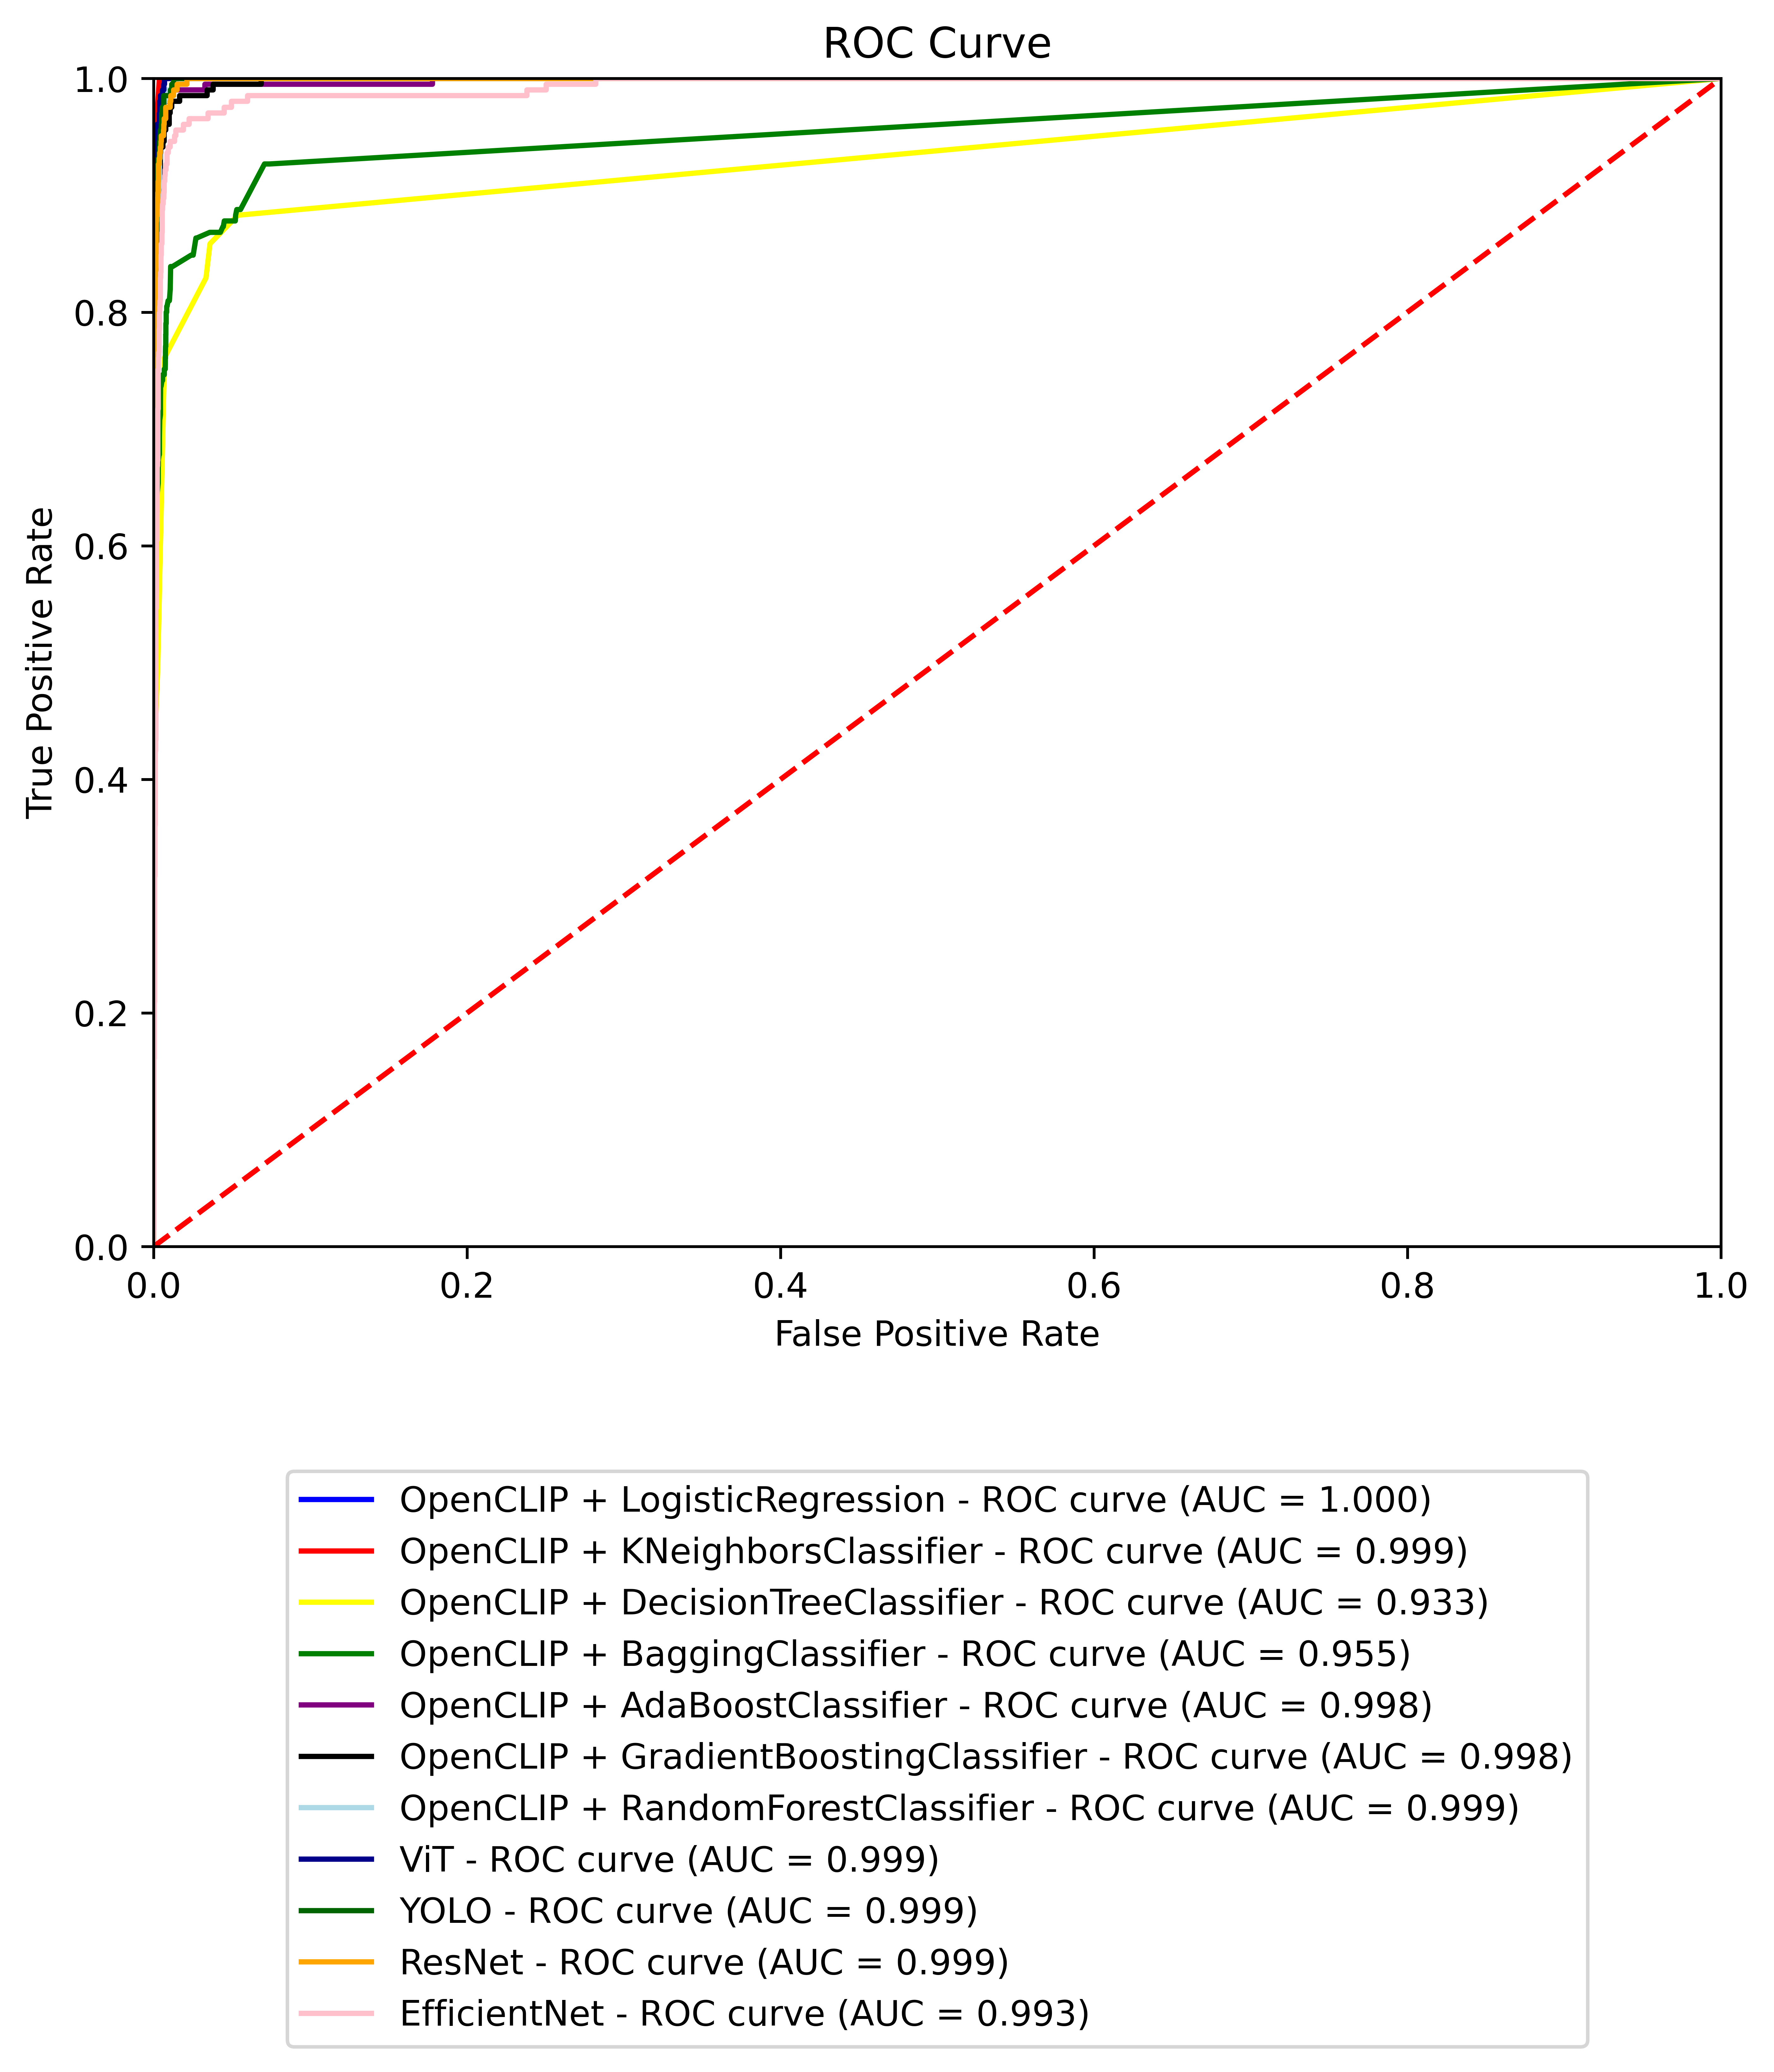
\includegraphics[width=0.8\textwidth]{figures/ROC}
  \caption{Receiver Operating Characteristic (ROC) curves for all models on the binary classification task, depicting the trade-off between true positive rate and false positive rate across classification thresholds.}
  \label{fig:roc-curve}
\end{figure}

\begin{figure}[ht]
  \centering
  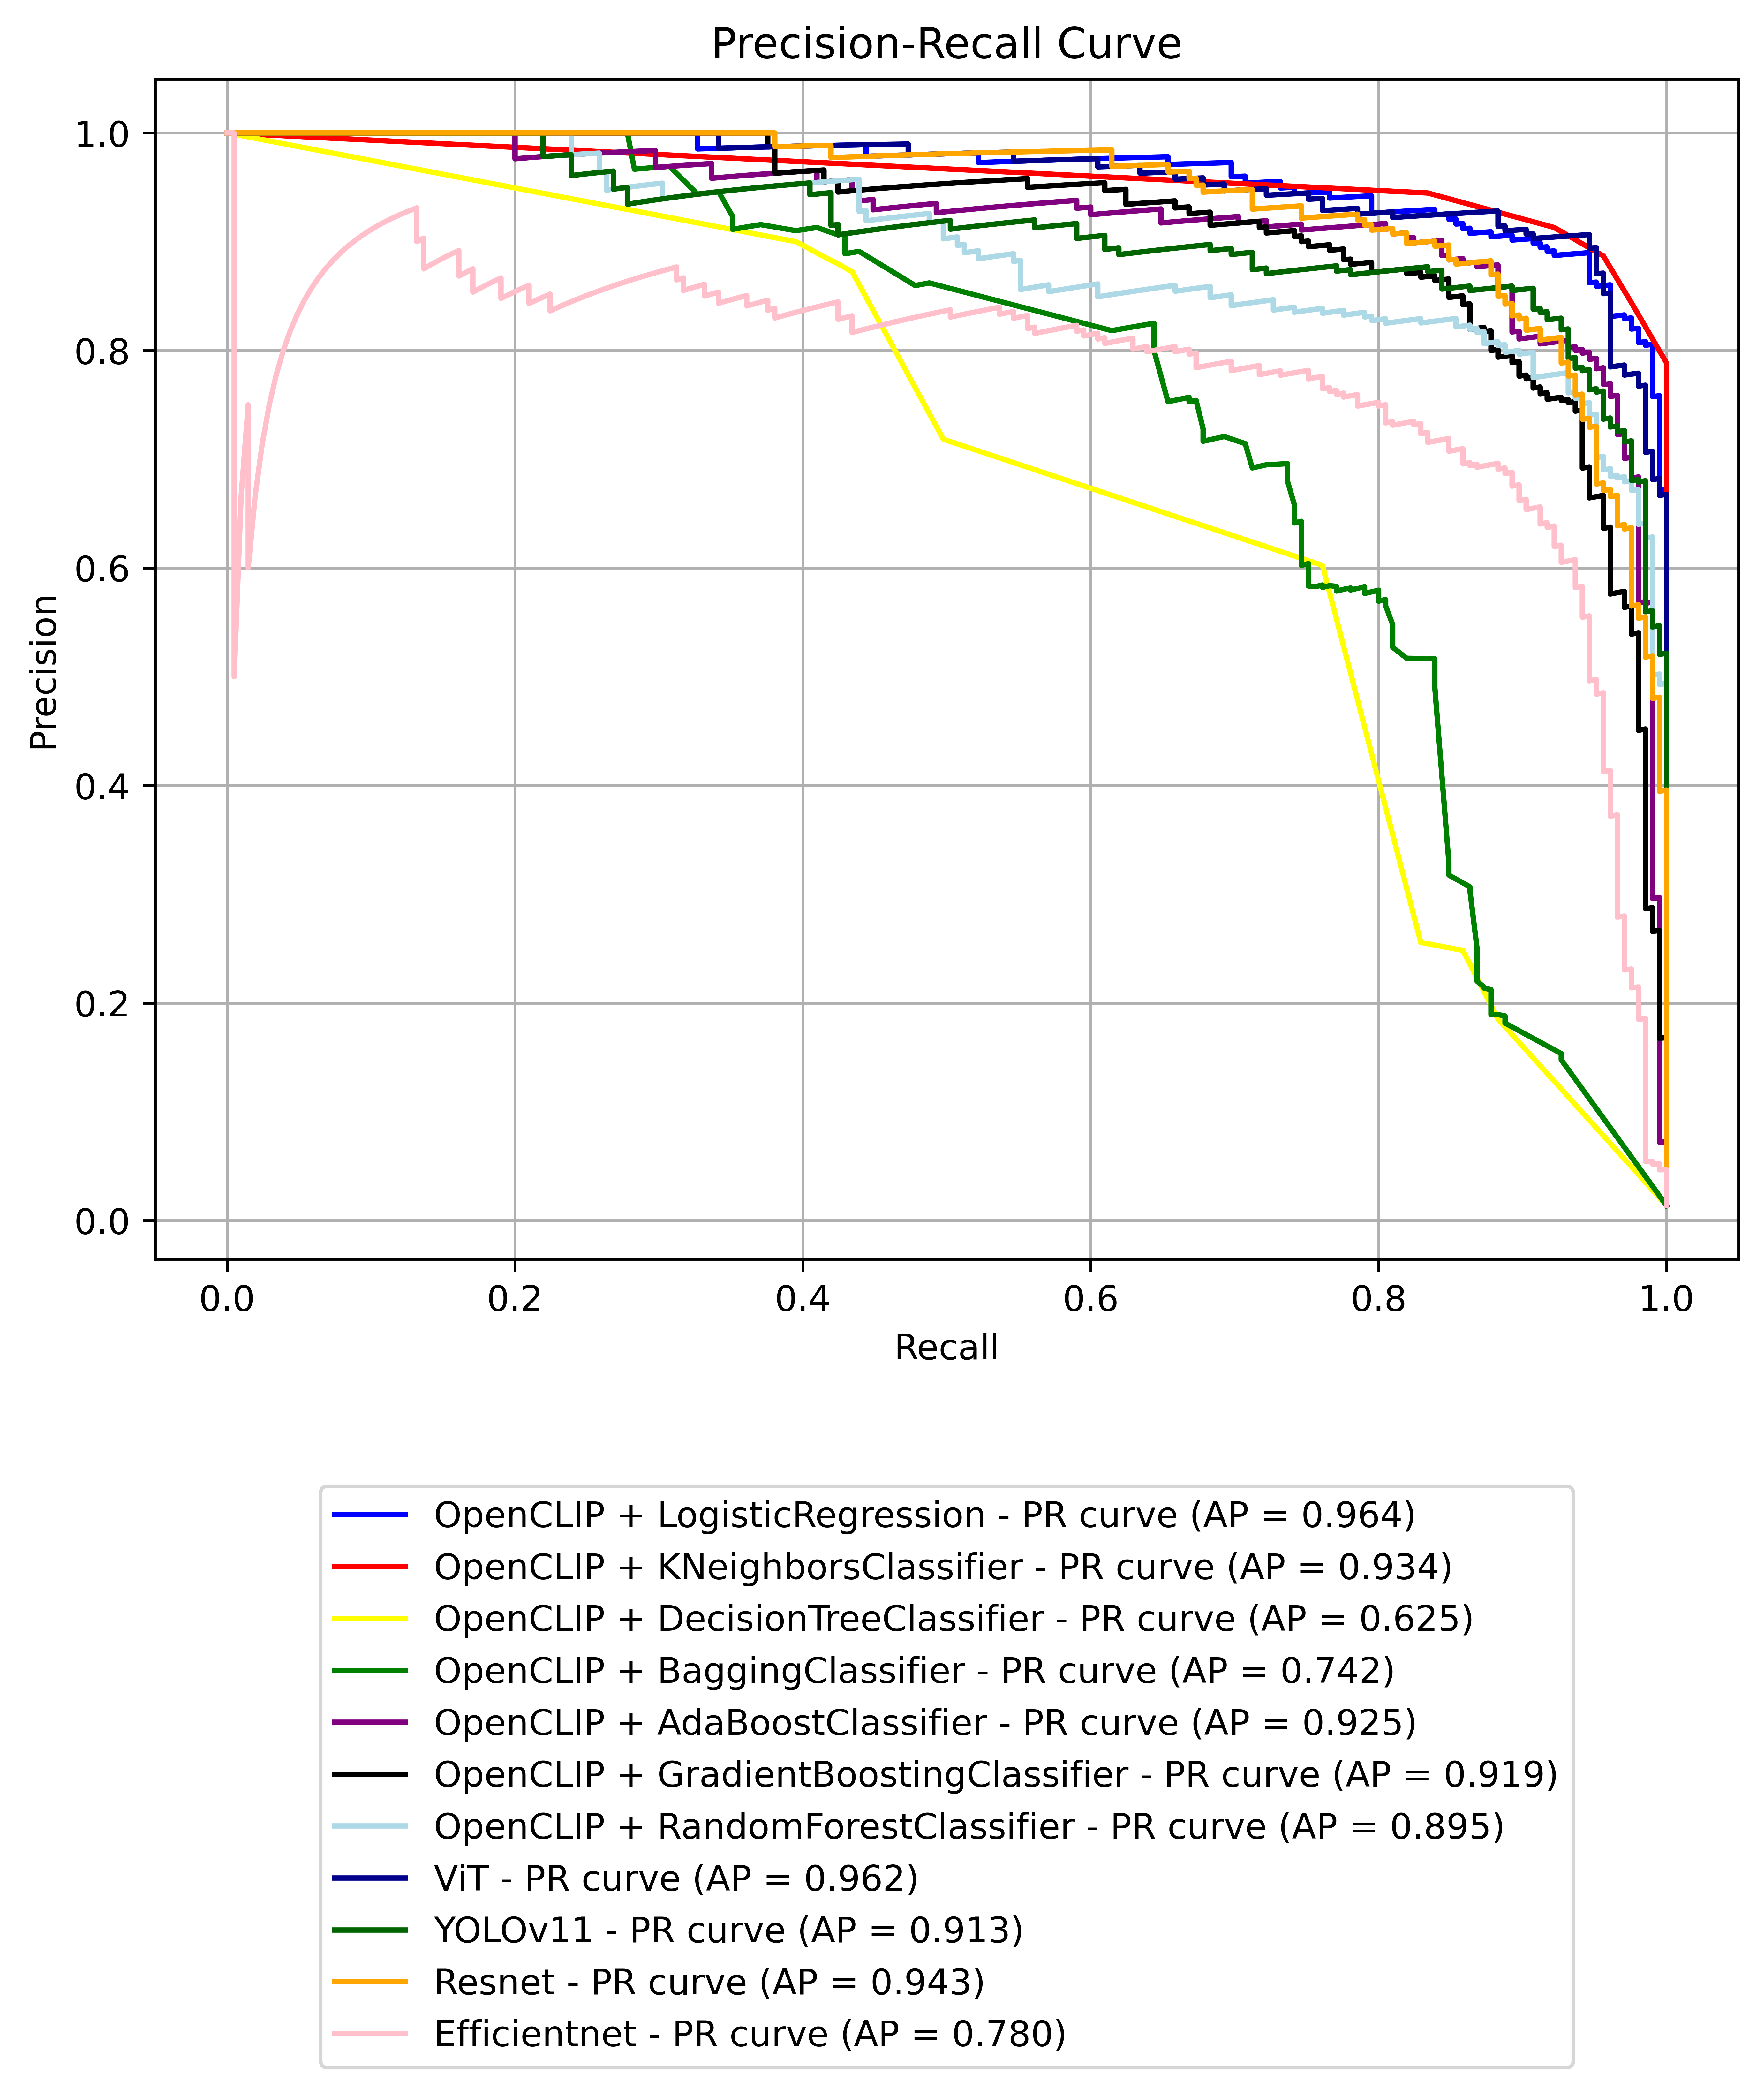
\includegraphics[width=0.8\textwidth]{figures/PR}
  \caption{Precision-Recall (PR) curves for all models on the binary classification task, highlighting model performance under class imbalance conditions.}
  \label{fig:pr-curve}
\end{figure}

\subsection{Reduced-Symbol Set Experiment}

To further evaluate model robustness, an additional experiment was conducted using a reduced set of Nazi symbols
from the original dataset. This subset included the three most visually distinct symbols: the \textit{SS Skull},
\textit{Siegrune}, and \textit{Swastika}.

The results of this reduced-symbol experiment are presented in ~\autoref{tab:binary-reduced-symbols-result},
indicating the models' performance when focusing on a smaller, more visually distinct set of classes.

%! Author = zhiweizhang
%! Date = 10.06.25

\begin{table}[ht]
  \centering
  \resizebox{\textwidth}{!}{
    \begin{tabular}{lccccc}
    \toprule
    \textbf{Model}                        & \textbf{Accuracy} & \textbf{Precision} & \textbf{Recall} & \textbf{F1-Score} \\
    \midrule
    YOLO                                  & 0.994             & 0.792              & 0.568           & 0.661             \\
    ResNet                                & 0.996             & 0.798              & 0.932           & 0.860             \\
    EfficientNet                          & 0.987             & 0.667              & 0.744           & 0.703             \\
    ViT                                   & \textbf{0.998}    & 0.972              & 0.926           & \textbf{0.948}    \\
    Moondream                             & 0.996             & 0.840              & 0.851           & 0.846             \\
    OpenCLIP                              & 0.864             & 0.025              & 0.338           & 0.047             \\
    OpenCLIP + Logistic Regression        & 0.996             & 0.917              & 0.835           & 0.874             \\
    OpenCLIP + SGDClassifier              & 0.996             & 0.899              & 0.895           & 0.897             \\
    OpenCLIP + KNeighborsClassifier       & \textbf{0.998}    & 0.895              & \textbf{0.989}  & 0.940             \\
    OpenCLIP + SVC                        & \textbf{0.998}    & \textbf{0.973}     & 0.900           & 0.935             \\
    OpenCLIP + DecisionTreeClassifier     & 0.985             & 0.514              & 0.635           & 0.568             \\
    OpenCLIP + BaggingClassifier          & 0.987             & 0.566              & 0.639           & 0.600             \\
    OpenCLIP + AdaBoostClassifier         & 0.994             & 0.869              & 0.742           & 0.800             \\
    OpenCLIP + GradientBoostingClassifier & 0.993             & 0.837              & 0.708           & 0.767             \\
    OpenCLIP + RandomForestClassifier     & 0.988             & 0.959              & 0.209           & 0.344             \\
    OpenCLIP + VotingClassifier           & 0.997             & 0.964              & 0.833           & 0.894             \\
    \bottomrule
    \end{tabular}
  }
  \caption{Binary classification performance across different models on reduced-symbol set. The best scores for each metric are highlighted in bold.}
  \label{tab:binary-reduced-symbols-result}
\end{table}

As expected, reducing the class set to visually distinct symbols improved performance across most models. This
demonstrates the impact of inter-class visual similarity on model accuracy. With fewer symbols and more training
samples per class, models could learn cleaner decision boundaries and avoid confusion between ambiguous or
similar-looking symbols.

Implications of improved results on the reduced symbol set, and their relevance to dataset complexity and model
robustness, are explored in more depth in the ~\autofullref{chapter:discussion-and-analysis}.


\section{Multi-Class Classification Results}

\subsection{Tabular Results}

The multi-class classification results are summarized in ~\autoref{tab:multi-class-results}, reporting
macro-averaged accuracy, precision, recall, and F1-score for each model.

%! Author = zhiweizhang
%! Date = 10.06.25

\begin{table}[ht]
\centering
\resizebox{\textwidth}{!}{
\begin{tabular}{lcccc}
\toprule
\textbf{Model}                        & \textbf{Accuracy (Macro)} & \textbf{Precision (Macro)} & \textbf{Recall (Macro)} & \textbf{F1-score (Macro)} \\
\midrule
YOLOv11                               & \textbf{0.884}            & \textbf{0.865}             & \textbf{0.818}          & \textbf{0.833}            \\
ResNet                                & 0.879                     & 0.850                      & 0.795                   & 0.810                     \\
EfficientNet                          & 0.794                     & 0.710                      & 0.697                   & 0.698                     \\
ViT                                   & 0.876                     & 0.833                      & 0.775                   & 0.790                     \\
Moondream                             & 0.608                     & 0.412                      & 0.601                   & 0.355                     \\
OpenCLIP                              & 0.274                     & 0.354                      & 0.413                   & 0.265                     \\
OpenCLIP + Logistic Regression        & 0.768                     & 0.476                      & 0.390                   & 0.412                     \\
OpenCLIP + SGDClassifier              & 0.799                     & 0.749                      & 0.624                   & 0.632                     \\
OpenCLIP + KNeighborsClassifier       & 0.752                     & 0.598                      & 0.518                   & 0.530                     \\
OpenCLIP + SVC                        & 0.815                     & 0.723                      & 0.593                   & 0.620                     \\
OpenCLIP + DecisionTreeClassifier     & 0.577                     & 0.177                      & 0.160                   & 0.154                     \\
OpenCLIP + BaggingClassifier          & 0.599                     & 0.320                      & 0.179                   & 0.177                     \\
OpenCLIP + AdaBoostClassifier         & 0.648                     & 0.404                      & 0.275                   & 0.305                     \\
OpenCLIP + GradientBoostingClassifier & 0.704                     & 0.444                      & 0.412                   & 0.389                     \\
OpenCLIP + RandomForestClassifier     & 0.583                     & 0.261                      & 0.162                   & 0.161                     \\
OpenCLIP + VotingClassifier           & 0.770                     & 0.481                      & 0.391                   & 0.415                     \\
\bottomrule
\end{tabular}
}
  \caption{Multi-class classification performance across different models. The best scores for each metric are highlighted in bold.}
\label{tab:multi-class-results}
\end{table}

\subsection{Visual Comparison}

~\autoref{fig:model-f1-score} \autoref{fig:model-accuracy}, \autoref{fig:model-precision}, and
\autoref{fig:model-recall} also include the multi-class classification results, presented on the right side of
each plot. These visualizations allow for direct comparison of model effectiveness across multiple symbol classes.

In this setting, \ac{YOLO} consistently outperformed other models across all evaluation metrics, followed closely by
\ac{ResNet} and \ac{ViT}, both of which demonstrated strong and consistent classification performance. Models such as
Moondream and OpenCLIP showed less consistent results across different classes.

\subsection{Confusion Matrices}

Confusion matrices for the multi-class classification task are shown in the figures below. Each matrix corresponds
to a model trained to classify images into one of thirteen symbol categories:

\begin{quote}
\texttt{['Black Sun', 'Flash and circle', 'Broken Sun Cross', 'The Happy Merchant', 'Hitler', 'Nazi salute',
  'Yellow badge', 'neo-Nazi', 'Siegrune', 'SS Skull', 'Sturmabteilung emblem', 'Swastika', 'Wolfsangel']}
\end{quote}

These matrices reveal class-specific performance, highlighting where misclassifications occur and identifying
classes that are frequently confused. Such insights assist in understanding model limitations and potential areas
for improvement.

\begin{itemize}
  \item \textbf{\ac{ResNet}:} Demonstrates strong performance on prominent symbols such as \textit{Swastika} and
  \textit{Siegrune}, with occasional confusion among visually similar classes.
  \item \textbf{\ac{YOLO}:} Achieves high accuracy on frequent classes but struggles with rarer symbols like
  \textit{Nazi salute} and \textit{Broken Sun Cross}. Overall, it has the best performance across all classes.
  \item \textbf{EfficientNet:} Yields balanced performance but exhibits reduced confidence on ambiguous or
  underrepresented categories.
  \item \textbf{\ac{ViT}:} Shows strong recognition for dominant classes, with some misclassifications on less
  frequent symbols.
  \item \textbf{OpenCLIP encoder + \ac{SVC}:} The text-image contrastive learning approach produces reasonable results,
  particularly for \textit{Swastika}, but is sensitive to class imbalance.
\end{itemize}

\input{figures/yolo_confusion_matrix_multiclass}
\input{figures/efficientnet_confusion_matrix_multiclass}
\input{figures/resnet_confusion_matrix_multiclass}
\input{figures/vit_confusion_matrix_multiclass}
%! Author = zhiweizhang
%! Date = 13.06.25

% Preamble
\begin{figure}[ht]
    \centering
    \begin{tikzpicture}
        \begin{axis}[
            colormap={bluewhite}{color=(white) rgb255=(90,96,191)},
            xlabel=Predicted,
            xlabel style={yshift=-10pt},
            ylabel=Actual,
            ylabel style={yshift=10pt},
            xticklabels={
                Black Sun,
                Flash and circle,
                Broken Sun Cross,
                The Happy Merchant,
                Hitler,
                Nazi salute,
                Yellow badge,
                Neo-Nazi,
                Siegrune,
                SS Skull,
                Sturmabteilung emblem,
                Swastika,
                Wolfsangel
            }, % changed
            xtick={0,...,12}, % changed
            xtick style={draw=none},
            yticklabels={
                Black Sun,
                Flash and circle,
                Broken Sun Cross,
                The Happy Merchant,
                Hitler,
                Nazi salute,
                Yellow badge,
                Neo-Nazi,
                Siegrune,
                SS Skull,
                Sturmabteilung emblem,
                Swastika,
                Wolfsangel
            }, % changed
            ytick={0,...,12}, % changed
            ytick style={draw=none},
            enlargelimits=false,
            colorbar,
%            colorbar style={
%              ytick={0, 0.5, 1.0, 1.5},
%              yticklabels={0, 0.5, 1.0, 1.5},
%%              xtick=\empty,
%%              ylabel style={yshift=10pt},
%            },
            point meta min=0,
            point meta max=100,
            xticklabel style={
              rotate=90,
            },
%            yticklabel style={
%              text width=1cm,align=center
%            },
            nodes near coords={\pgfmathprintnumber\pgfplotspointmeta},
            nodes near coords style={
                yshift=-7pt
            },
        ]
            \addplot[
                matrix plot,
                mesh/cols=13, % changed
                point meta=explicit,
                draw=gray
            ] table [meta=C, x=x, y=y, col sep=comma] {data/openclip_encoder-multiclass-confusion-matrix-data.csv};
        \end{axis}
    \end{tikzpicture}
    \caption{Confusion matrix for the binary classification task using OpenCLIP encoder and SVC. The values represent the number of samples in each cell.}
    \label{fig:openclip-encoder-confusion-matrix-multiple}
\end{figure}

Across multi-class results, \textbf{YOLO} stands out as the top performer. Its architecture enables spatial
attention and object localization, making it well-suited to distinguish between overlapping or co-located symbols.
In contrast, \textbf{ViT} and \textbf{ResNet} rely on whole-image representations and struggle more with occlusion
or background noise.

Moondream and vanilla OpenCLIP again performed poorly, reinforcing that general-purpose vision-language models are
not optimal for fine-grained symbol classification—especially without prompt engineering or task-specific tuning.

Detailed analysis and interpretation of multi-class classification challenges and model behaviors are deferred to
the ~\autofullref{chapter:discussion-and-analysis}.